
%----------------------------------------------------------------------------------------
%	PACKAGES AND OTHER DOCUMENT CONFIGURATIONS
%----------------------------------------------------------------------------------------

\documentclass[
10pt, % Main document font size
a4paper, % Paper type, use 'letterpaper' for US Letter paper
oneside, % One page layout (no page indentation)
%twoside, % Two page layout (page indentation for binding and different headers)
headinclude,footinclude, % Extra spacing for the header and footer
BCOR5mm, % Binding correction
]{report}

%%%%%%%%%%%%%%%%%%%%%%%%%%%%%%%%%%%%%%%%%
% Arsclassica Article
% Structure Specification File
%
% This file has been downloaded from:
% http://www.LaTeXTemplates.com
%
% Original author:
% Lorenzo Pantieri (http://www.lorenzopantieri.net) with extensive modifications by:
% Vel (vel@latextemplates.com)
%
% License:
% CC BY-NC-SA 3.0 (http://creativecommons.org/licenses/by-nc-sa/3.0/)
%
%%%%%%%%%%%%%%%%%%%%%%%%%%%%%%%%%%%%%%%%%

%----------------------------------------------------------------------------------------
%	REQUIRED PACKAGES
%----------------------------------------------------------------------------------------

\usepackage[
nochapters, % Turn off chapters since this is an article        
beramono, % Use the Bera Mono font for monospaced text (\texttt)
eulermath,% Use the Euler font for mathematics
pdfspacing, % Makes use of pdftex’ letter spacing capabilities via the microtype package
dottedtoc % Dotted lines leading to the page numbers in the table of contents
]{classicthesis} % The layout is based on the Classic Thesis style

\usepackage{arsclassica} % Modifies the Classic Thesis package

\usepackage[T1]{fontenc} % Use 8-bit encoding that has 256 glyphs

\usepackage[utf8]{inputenc} % Required for including letters with accents

\usepackage{graphicx} % Required for including images
\graphicspath{{Figures/}} % Set the default folder for images

\usepackage{enumitem} % Required for manipulating the whitespace between and within lists

\usepackage{lipsum} % Used for inserting dummy 'Lorem ipsum' text into the template

\usepackage{subfig} % Required for creating figures with multiple parts (subfigures)

\usepackage{amsmath,amssymb,amsthm} % For including math equations, theorems, symbols, etc

\usepackage{varioref} % More descriptive referencing

\usepackage[francais]{babel}

\usepackage{cite}

\usepackage{natbib}

%----------------------------------------------------------------------------------------
%	THEOREM STYLES
%---------------------------------------------------------------------------------------

\theoremstyle{definition} % Define theorem styles here based on the definition style (used for definitions and examples)
\newtheorem{definition}{Definition}

\theoremstyle{plain} % Define theorem styles here based on the plain style (used for theorems, lemmas, propositions)
\newtheorem{theorem}{Theorem}

\theoremstyle{remark} % Define theorem styles here based on the remark style (used for remarks and notes)

%----------------------------------------------------------------------------------------
%	HYPERLINKS
%---------------------------------------------------------------------------------------

\hypersetup{
%draft, % Uncomment to remove all links (useful for printing in black and white)
colorlinks=true, breaklinks=true, bookmarks=true,bookmarksnumbered,
urlcolor=webbrown, linkcolor=RoyalBlue, citecolor=webgreen, % Link colors
pdftitle={}, % PDF title
pdfauthor={\textcopyright}, % PDF Author
pdfsubject={}, % PDF Subject
pdfkeywords={}, % PDF Keywords
pdfcreator={pdfLaTeX}, % PDF Creator
pdfproducer={LaTeX with hyperref and ClassicThesis} % PDF producer
} % Include the structure.tex file which specified the document structure and layout

\hyphenation{Fortran hy-phen-ation} % Specify custom hyphenation points in words with dashes where you would like hyphenation to occur, or alternatively, don't put any dashes in a word to stop hyphenation altogether

%----------------------------------------------------------------------------------------
%	TITLE AND AUTHOR(S)
%----------------------------------------------------------------------------------------

\title{\normalfont\spacedallcaps{Faut-il tester le code ou les modèles de composants logiciels ?}} % The article title

\date{} % An optional date to appear under the author(s)

%----------------------------------------------------------------------------------------

\newcommand{\HRule}{\rule{\linewidth}{0.5mm}}

\addto\captionsfrench{% Replace "english" with the language you use
  \renewcommand{\contentsname}
    {Sommaire}
}

\begin{document}

\begin{titlepage}
	\begin{sffamily}
		\begin{center}
																																										
			% Upper part of the page. The '~' is needed because \\
			% only works if a paragraph has started.
			
\includegraphics[scale=0.2]{Figures/univnantes.png}~\\[1.5cm]
																																																								
				\textsc{\LARGE Université de Nantes}\\[0.5cm]
				\textsc{\Large Master Informatique}\\[2cm]
				\textsc{\Large Rapport de stage TER}\\[1.5cm]
																																																								
				% Title
				\HRule \\[0.4cm]
				{ \huge \bfseries Faut-il tester le code ou les modèles de composants logiciels ?\\[0.4cm] }
																																																								
				\HRule \\[3cm]
				%\includegraphics[scale=0.2]{Figures/Dolor.JPG}
				%\\[2cm]
																																																								
				% Author and supervisor
				\begin{minipage}{\textwidth}
					\begin{flushleft} \large
						\textsc{\Large Réalisé par : } \\
						Daniel \textsc{Ahmed}\\
						Yamen \textsc{Alnajm}\\
						Soufyane \textsc{Belhadj Kacem}\\
						Promo 2018\\
					\end{flushleft}
				\end{minipage}
				\begin{minipage}{\textwidth}
					\begin{flushright} \large
						\emph{Tuteur :} \\
						M. \textsc{Gilles Ardourel}\\
						M. \textsc{Pascal Andre}\\
						M. \textsc{Jean-Marie Mottu}\\
						\emph{Chef d'équipe : } \\
						M. \textsc{Gile}
					\end{flushright}
				\end{minipage}
																																																								
				\vfill
																																																								
				% Bottom of the page
				%{\large 1\ier{} Juillet 2013 — 30 Août 2013}
																																																								
			\end{center}
		\end{sffamily}
	\end{titlepage}
								  
	%----------------------------------------------------------------------------------------
	%	HEADERS
	%----------------------------------------------------------------------------------------
												
	\renewcommand{\sectionmark}[1]{\markright{\spacedlowsmallcaps{#1}}} % The header for all pages (oneside) or for even pages (twoside)
	\renewcommand{\subsectionmark}[1]{\markright{\thesubsection~#1}} % Uncomment when using the twoside option - this modifies the header on odd pages
	\lehead{\mbox{\llap{\small\thepage\kern1em\color{halfgray} \vline}\color{halfgray}\hspace{0.5em}\rightmark\hfil}} % The header style
														
	\pagestyle{scrheadings} % Enable the headers specified in this block
	%----------------------------------------------------------------------------------------
	%	Fin HEADERS
	%----------------------------------------------------------------------------------------				
								  
	%----------------------------------------------------------------------------------------  
	% Remerciments					
	%----------------------------------------------------------------------------------------
														
	\newpage
	\section*{Remerciements} 
	Nous tenons  à remercier cordialement toutes les personnes qui nous ont permis de réaliser ce travail dans les meilleures conditions.\\ 
														
	Un remerciement particulier à Mr. Gilles ARDOUREL et Pascal ANDRÉ, nos enseignants responsables, pour nous avoir encadrés tout au long de ce travail. Merci pour leurs conseils, leurs disponibilités et leurs implications. \\
														
	Nous remercions les membres du jury qui ont bien voulu examiner et évaluer ce rapport.
	%----------------------------------------------------------------------------------------  
	%Fin Remerciments					
	%----------------------------------------------------------------------------------------  
								
	%----------------------------------------------------------------------------------------  
	%	ABSTRACT
	%----------------------------------------------------------------------------------------
								  
	\newpage
	\section*{Résumé}
														
	Ce sujet de rapport vise à étudier et appliquer l'approche d'ingénierie dirigée par les modèles pour le développement d’une application qui automatise les tests  logiciels au niveau du modèle.
	Le Budget IT consacrée aux tests et à l’assurance qualité augmente de 9 points d’une année sur l’autre, pour atteindre 35 \% de la dépense IT selon Capgemini. Contre seulement 26 \% en 2014 ! Et 18 \% en 2012.
														
	La SSII prévoit qu’en 2018, la part des tests et de la qualité passera à 40 \% du total. Ce budget colossal est divisé en parts égales entre maintenance d’applications existantes et nouveaux développement. Dans 35 \% des entreprises, cette inflation est considérée comme un problème \citep{silicon}.
														
	Cette problématique pousse les entreprises à adopter une nouvelle stratégie et de miser sur la recherche d’un mécanisme d’automatisation des tests logiciels.
														
	Cela nous ramène à penser à une solution pour automatiser les tests logiciel au niveau modèle, en se basant sur l’approche MDA, le but est d’offrir une interface qui donne la possibilité à l’utilisateur de choisir les composants ainsi que les services qui veulent tester, et notre application se charge du reste.\\
														
	Toute la partie de développement de ce projet fut mis en place de manière itérative, basée sur la méthodologie Agile.
	\section*{Mots-clés : Composants, Services, Modèles, Test, MDA}
														
	\newpage
	\section*{Abstract} 
	\lipsum[1]
								  
	%----------------------------------------------------------------------------------------						
	% Fin abstract
	%----------------------------------------------------------------------------------------
								
	%----------------------------------------------------------------------------------------  
	%Debut avant propos
	%----------------------------------------------------------------------------------------
								
	\newpage
	\section*{L’AVANT-PROPOS} 
	L’une des grandes craintes des dirigeants et chefs de projet est de constater une série de bugs sur le produit fini, les conséquences peuvent être désastreuse, comme une grande perte financière ou voir pire humaine.  
	La volonté de créer des applications de qualitées à amener les entreprises à repenser leurs façon de faire, et à automatiser les tests logiciel. Entre 2014 et 2015 le pourcentage de test automatisé est passé de 28% à 45%.
	Dans le cadre d’un thème de projet de stage proposé par l’équipe AELOS du laboratoire LS2N à Nantes, une (// a voir selon l’avancement) a été développé et délivré. 
	Ce rapport fournit toutes les informations concernant l’approche MDA et (// a voir selon l’avancement)
	%----------------------------------------------------------------------------------------  
	%Fin avant propos
	%----------------------------------------------------------------------------------------
								 
	%----------------------------------------------------------------------------------------    
	%Debut tableofcontents 
	%----------------------------------------------------------------------------------------
								  
	\newpage			
	%\setcounter{tocdepth}{2} % Set the depth of the table of contents to show sections and subsections only
	\dominitoc[n]		
	\tableofcontents 
								  
	%----------------------------------------------------------------------------------------  
	%Fin tableofcontents 
	%----------------------------------------------------------------------------------------
								  
														
	%----------------------------------------------------------------------------------------  
	%	INTRODUCTION
	%----------------------------------------------------------------------------------------
								  
  \newpage
	\section{Introduction}
	Dans le développement dirigé par les modèles (MDD), il est essentiel de s’assurer de la correction des modèles avant de commencer le processus de transformations et de génération de codes. On diminue ainsi le coût élevé de la détection tardive d’erreurs. l’équipe que nous avons intégrée durant ce stage “AeLoS” travaille sur la vérification et la validation de logiciels aux niveaux modèles.
														    
	Le test est un moyen très utilisé pour vérifier et valider les applications, mais ce dernier rencontre plusieurs problèmes comme la couverture des tests, l’hétérogénéité du code, séparation des points de vue…
														    
	En 2013, l’équipe AELOS à réaliser des travaux sur l’assistance à la construction du harnais de tests, en 2014 et 2015, le prototype a été amélioré par des groupes d’étudiants du Master Alma. En 2018 nous reprenons le projet afin d'expérimenter une nouvelle approche, le cas d'études se portera sur le contrôle de voiture autonome.
	%----------------------------------------------------------------------------------------
	%Fin introduction
	%----------------------------------------------------------------------------------------
								
	%----------------------------------------------------------------------------------------  
	% Chapitre 1 debut
	%----------------------------------------------------------------------------------------
								  
	\newpage
	\chapter{Chapitre 1 : vérification des systèmes à composant}
	\minitoc
	\section{Introduction}
	\lipsum[5] % Dummy text	
	\section{L'outil Kmelia}
	\lipsum[5] % Dummy text
	\section{L'architecture du système}
	\lipsum[5] % Dummy text
	\section{L'outil CostoTest}
	\lipsum[5] % Dummy text
	\section{Conclusion}
	\lipsum[10]		
								  
	%----------------------------------------------------------------------------------------  
	% Chapitre 1 Fin
	%----------------------------------------------------------------------------------------					
														
	%----------------------------------------------------------------------------------------											
	%Chapitre 2 debut					
	%----------------------------------------------------------------------------------------					
														
	\newpage 
	\chapter{Chapitre 2 : ingénierie dirigé par les model}
	\minitoc  
	\section{Introduction}
    Pour  bien manipuler les composants nous utiliserons l’approche d'ingénierie dirigée par les modèles MDA, que nous allons présenter dans ce chapitre.
    L’ingénierie  des systèmes informatiques se base sur les modèles. Ces modèles permettent de décrire les systèmes en cours de développement et leur environnement à différents niveaux d’abstractions. Ces abstractions permettent de concevoir des applications indépendantes des plate-formes cibles. 
    L’approche de l’ingénierie dirigée par les Modèles (IDM) consiste à programmer au niveau des modèles, représentés ces derniers comme une instance d’un méta-modèle, et à les utiliser pour générer le code final des applications.\\[1.5cm]
    
    \begin{figure}[H] 
    \centering     
		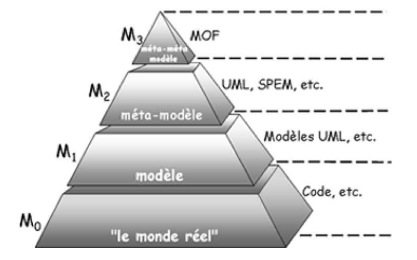
\includegraphics[scale=0.8]{Figures/Pyramide_de_modelisation.png}
		\caption{Pyramide de modélisation de l'OMG \citep{PyramideMDA}}
		\end{figure}  
    
    Le MDA (Model Driven Architecture) de l’OMG est une approche typique d’ingénierie dirigée par les modèles pour la conception d’application, elle est basée sur le standard UML pour la définition des modèles et sur l’environnement de méta-méta modélisation MOF (Meta Object Facility) pour la programmation au niveau modèle et la génération de codes.
		L'ingénierie dirigée par les modèles est donc un paradigme dans lequel la modélisation est considérée comme l'élément central d'un logiciel.   
					
		\section{Les modèles MDA et ses transformations}
					
		\subsection{Les modèles MDA}
		\subsubsection{ CIM : Computation Independent Model }
		Les  modèles d'exigence CIM décrivent les besoins fonctionnels de l'application, aussi bien les services qu'elle offre et les entités avec lesquelles elle interagit. Les CIM peuvent servir de référence pour s'assurer que l'application finie correspond aux demandes des clients.
		\subsubsection{ PIM : Platform Independent Model}
		Les modèles d’analyse et de conception de l’application PIM représentent, indépendamment de toute plate-forme technique, une  spécification neutre d'un système (modèle de métier et de service) qui ignore tous les détails de mise en œuvre et d’utilisation du système décrit.
		\subsubsection{PSM  : Platform Specific Model}
		Les modèles de code PSM sont des modèles de métier et de service liés  à une ou plusieurs plate-formes d’exécution.
		\subsubsection{Code source}
		Le code source est le résultat final de tout le processus MDA, il est généré automatiquement à partir du modèle PSM.
		\section{Les transformations de modèles}
		Le passage de PIM à PSM fait intervenir des mécanismes de transformation de modèles. La transformation de modèles est le processus qui convertit un modèle en un autre modèle.
		L'approche  MDA demande de créer d'abord un modèle d’analyse (PIM), ce dernier est raffiné en un ou plusieurs modèles spécifiques à une ou plusieurs (PSM). 
    La transformation du PIM vers PSM peut être complétée par d’autres informations comme celles relative au mapping entre le PIM et le PSM ou à la description de la plate-forme (PDM).
    
				
    \section{Les objectifs du MDA }
    L’approche MDA de l’OMG a été défini pour répondre aux problèmes liés à l’évaluation continue des technologies, parmi les objectifs de cette approche : 
    \subsubsection{Les modèles pérennes :}
    L’objectif  majeur du MDA est l’élaboration des modèles pérennes (PIM), ces derniers doivent survivre le changement de plate-forme et être réutilisable pour plusieurs plate-formes.
        Cette  pérennité est garantie  grâce à l'utilisation d'UML qui est un standard stable mais aussi grâce  aux modèles qui sont par nature des entités pérennes.
    \subsubsection{Les gains de productivité :}
    Les modèles sont la base du processus MDA, ils facilitent la communication entre experts du domaine et développeurs. Dans cette approche les modèles sont considérés comme un  outil de production à l’aide de l'automatisation des transformations de modèles.
    La génération de la totalité de modèles de  code (PSM) devient alors automatique, à cause des modèles qui sont  considérés comme des  éléments qui véhiculent une information précise est nécessaire pour cette transformation. Le mappage automatique de la PSM permet  d'enlever le risque d'erreur, il produit ainsi un gain de coût à la transformation de la PIM, c’est le gain de productivité. 
    \subsubsection{La prise en compte des plate-forme d'exécution :}	
    La  MDA  permet d’intégrer  les spécifications des différentes plate-formes d'exécution pendant la transformation du modèle PIM vers PSM.  Et de cette manière le développement des applications mobiles multi-plateformes est devenu facile, puisque tout est basé sur un modèle PIM qui est indépendant des détails techniques des plate-formes d’exécution (J2EE, .Net, PHP, etc.)
    Il  faut  noter  que toutes  modifications  dans le  modèle PIM, conduit à un changement dans les fonctionnalités du système livré.

		\section{Conclusion}
		Dans ce chapitre nous avons détaillé l’approche d'ingénierie dirigée par les modèles MDA, mais ce n'est pas la seule approche de génie logiciel qui se base sur les modèles dans son processus de développement. 
										  
		%----------------------------------------------------------------------------------------					  
		%Chapitre 2 fin					
		%----------------------------------------------------------------------------------------					
										  
		%----------------------------------------------------------------------------------------					  						
		%Chapitre 3 debut
		%----------------------------------------------------------------------------------------					
										  
		\newpage 
		\chapter{Chapitre 3 : intention de test et assemblage}
		\minitoc  
		\section{Introduction}
		\lipsum[5] % Dummy text
		\section{L'intention de test}
		\lipsum[5] % Dummy text
		\section{Architecture}
		\lipsum[5] % Dummy text
		\section{L'assistance au harnais de test}
		\lipsum[5] % Dummy text
		\section{Conclusion}
		\lipsum[10]	
										  
		%----------------------------------------------------------------------------------------					  
		%Chapitre 3 fin
		%----------------------------------------------------------------------------------------					  
										  
		%----------------------------------------------------------------------------------------					  
		%Chapitre 4 debut
		%----------------------------------------------------------------------------------------					
										  
		\newpage 
		\chapter{Chapitre 4 : transformation des models xtext}
		\minitoc  
		\section{Introduction}
		\lipsum[10] % Dummy text
		\section{Conclusion}
		\lipsum[10]
										  
		%----------------------------------------------------------------------------------------					  
		%Chapitre 4 fin  
		%----------------------------------------------------------------------------------------					
										  
		%----------------------------------------------------------------------------------------					  
		%Chapitre 5 debut
		%----------------------------------------------------------------------------------------					
										  
		\newpage
		\chapter{Chapitre 5 : Application de la méthode proposée  }
		\minitoc  
		\section{Introduction}
		\lipsum[10]
		\section{Processus de développement}
		Derouler un exemple.....
		\section{Evaluation}
		Ce que nous avons réussi, a faire et a ne pas faire
		\section{Conclusion}
		\lipsum[10]	
										  
		%----------------------------------------------------------------------------------------					  
		%Chapitre 5 fin
		%----------------------------------------------------------------------------------------					  
										  
		%----------------------------------------------------------------------------------------					  
		%debut conclusion generale
		%----------------------------------------------------------------------------------------					
										  
		\newpage
		\section{CONCLUSION GENERALE}
		\subsection{Conclusion}
		\lipsum[10]
		\subsection{Perspectives}
		\lipsum[10]
										  
		%----------------------------------------------------------------------------------------					  
		%fin conclusion generale
		%----------------------------------------------------------------------------------------					
										  
														  
		%----------------------------------------------------------------------------------------
		%	TABLE OF CONTENTS & LISTS OF FIGURES AND TABLES
		%----------------------------------------------------------------------------------------
																
		\newpage
		\listoffigures % Print the list of figures
		\newpage
		\listoftables % Print the list of tables
										  
		%----------------------------------------------------------------------------------------
		%	Fin TABLE OF CONTENTS & LISTS OF FIGURES AND TABLES
		%----------------------------------------------------------------------------------------
											
																
		%----------------------------------------------------------------------------------------
		%	BIBLIOGRAPHY
		%----------------------------------------------------------------------------------------
																
		\renewcommand{\refname}{\spacedlowsmallcaps{References}} % For modifying the bibliography heading
		\newpage 
		\bibliographystyle{unsrt}
																
		\bibliography{biblio.bib} % The file containing the bibliography
																
		%----------------------------------------------------------------------------------------
		%	Fin BIBLIOGRAPHY
		%----------------------------------------------------------------------------------------
																
\end{document}